\documentclass[12pt, a4paper]{article}
\usepackage{cirilica}
\usepackage{geometry}
\usepackage{graphicx}
\usepackage{indentfirst}
\usepackage{multicol}

\geometry{
top=2cm,
right=2cm,
bottom=2cm,
left=2cm
}

\title{\lat{Latex}}
\author{Lazar Vukadinovi\' c}
\date{21. april 2024.}

\pagestyle{myheadings}
\markright{Primer dokumenta}

\begin{document}
    \maketitle
    \thispagestyle{empty}
    \newpage
    
    \section{Matematika}
    \subsection{Furijeova analiza}
    Svaka periodi?na funkcija\footnote{pogledati kako se definise funkcija}, po teoriji Furijeovih redova, mo�e se predstaviti pomo?u beskona?no monogo ortogonalnih funkcija. Kako ovaj na?in predstavljanja funkcije pru�a mogu?nost sasvim druga?ije analize u odnosu na analizu u vremenskom domenu, postavlja se pitanje da li je mogu?e istu ideju pro�iriti na funkcije koje nisu periodi?ne. Ako se neperiodi?na funkcija posmatra kao periodi?na sa beskona?no velikim periodom, Furijeova transformacija pro�iruje ovaj koncept razlaganja funkcija i na neperiodi?ne funkcije.
    
    \subsubsection{Formule}
    \begin{enumerate}
        \item Periodicne funkcije $f(x)=f(x+2\pi)$
        \item Predstavljanje: $a \cos{\omega x}  + b \sin{\omega x} \, a,b\in \mathbf{R}$
        \item $\prod_{i=N}^N=f(i)$
    \end{enumerate}
    
    \section{Modelovanje tema}
    \begin{multicols}{2}
        {\lat \itshape{Latent Dirichlet Allocation}}, nadalje {\lat{LDA}}, je najjednostavniji pristup problemu modelovanja tema   i njegova primena je predmet ovog rada.
        Osnovna karakteristika {\lat LDA} algoritma je mogu?nost  \textbf{izdvajanja} tema koje su prisutne u nekoj kolekciji dokumenata bez bilo kakvog dodatnog znanja. Dakle, primenom {\lat LDA}-a mogu?e je otkriti teme "o kojima govori" zadati skup dokumenata a da se pritom nikakvo dodatno ekspertsko znanje ne uklju?uje.
        Polazna pretpostavka {\lat LDA}-a je da svaki dokument u kolekciji dokumenata "govori o" vi�e tema. Opravdanost ove pretpostavke bi?e ilustrovana na nekoliko primera.
        Dobro je poznat roman Branka ?opi?a "Orlovi rano lete". Ukoliko bi neko ko nije pro?itao ovi knjigu �eleo da zna "o ?emu se radi" u njoj, najverovatnije bi dobio odgovor da je u pitanju knjiga koja se bavi do�ivljajima grupe de?aka na po?etku Drugog svetskog rata. Iako je to naj�iri okvir romana, u njemu su prisutne i teme o ljubavi, dru�enju, prijateljstvu, ratu, pustolovinama itd. Prema tome, roman, op�te gledano, obuhvata vi�e tema, ali se sa nekoliko njih intenzivno bavi.
    \end{multicols}
    
    \subsection{Graficki primer dokumenta}
    Generalno, proces zaklju?ivanja tematike dokumenta mo�e se ilustrovati slede?im primerom.
    Na Slici \ref{fig:tmSlika1}  predstavljen je ?lanak  Seeking Life's Bare(Genetic) Necessities koji govori o upotrebi analize podataka za odre?ivanje broja gena koji organizam treba da poseduje da bi pre�iveo (u evolutivnom smislu). Mo�e se uo?iti da su tri najzastupljenije oblasti u ovom tekstu - analiza podataka, evolutivna biologija i genetika. Na slici su ru?no ozna?ene neke re?i koje pripadaju ovim oblastima. Re?i koje se mogu svrstati u oblast   \textit{analize podataka} ozna?ene su plavom bojom, re?i koje pripadaju   \textit{genetici} ozna?ene su �utom bojom, dok su re?i koje se odnose na   \textit{evolutivnu biologiju} ozna?ene roze bojom. Ukoliko bi se ova procedura primenila na svaku re? teksta, jasno bi se uo?ilo koliko je koja tema zastupljena u ovom tekstu. Matemati?ki,   \textit{prisustvo} teme u tekstu se ozna?ava odnosom broja re?i "obojenih" datom bojom i ukupnog broja re?i u tekstu.
    
    \begin{figure}[h!]
    \centering
    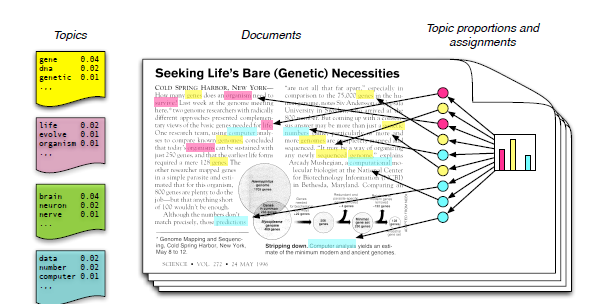
\includegraphics[scale=0.7]{tm.png}
    \caption{Primer clankova}
    \label{fig:tmSlika1}
    \end{figure}
    
    Naravno, postoje re?i koje se mogu svrstati u vi�e od jedne teme. Takve re?i bi bile obojene sa dve ili vi�e boja, ali zbog preglednosti slike, takvi slu?ajevi su izostavljeni.
    
    \newpage
    \subsection{Prikaz rada algoritama}
    Rad algoritama prikazanog na Slici \ref{fig:tmSlika1} je sledeci
    \begin{enumerate}
        \item Prvi korak: 
            \begin{center}
                \begin{tabular}{|c|c|c|c|c|}
                \hline
                    \multicolumn{5}{|c|}{Primer dokumenta}\\
                    \hline
                    & & & & \\
                    \hline
                    matematika & fizika & hemija & biologija & istorija \\
                    \hline
                \end{tabular}
            \end{center}
        \item Drugi korak:
            \begin{center}
                \begin{tabular}{|c|c|c|c|c|}
                \hline
                    \multicolumn{5}{|c|}{Primer dokumenta}\\
                    \hline
                    $\sum_1^N{f(reci)}$ & $\sum_1^N{f(reci)}$ & $\sum_1^N{f(reci)}$ & $\sum_1^N{f(reci)}$ & $\sum_1^N{f(reci)}$ \\
                    \hline
                    matematika & fizika & hemija & biologija & istorija \\
                    \hline
                \end{tabular}
            \end{center}
        \item Finalni korak:
            \begin{center}
                \begin{tabular}{|c|c|c|c|}
                \hline
                    Reci & \multicolumn{3}{|c|}{Teme}\\
                    \hline \hline
                    & 1 & 2 & 3 \\
                    \hline
                    matematika & $n_1^1$ & $n_2^1$ & $n_3^1$ \\
                    \hline
                    fizika & $n_1^2$ & $n_2^2$ & $n_3^2$ \\
                    \hline
                    hemija & $n_1^3$ & $n_2^3$ & $n_3^3$ \\
                    \hline
                    biologija & $n_1^4$ & $n_2^4$ & $n_3^4$ \\
                    \hline
                    istorija & $n_1^5$ & $n_2^5$ & $n_3^5$ \\
                    \hline
                    \hline
                \end{tabular}
            \end{center}
    \end{enumerate}
    
    \begin{thebibliography}{99}
    \bibitem{mell} {\lat Mell, Peter, and Tim Grance. The NIST definition of cloud computing. (2011).}
    \bibitem{buyya} {\lat Buyya, Rajkumar, et al. Cloud computing and emerging IT platforms: Vision, hype, and reality for delivering computing as the 5th utility."Future Generation computer systems 25.6 (2009): 599-616.}
    \end{thebibliography}
    
    \newpage
    \tableofcontents
    \thispagestyle{empty}
\end{document}